\chapter{Neural Network Noise Suppression}\label{NeuralNetworkNoiseSuppression}
In this section the Machine learning approach will be explained together with the signal processing needed for it.
This method will be used to suppress the noise from the signal, keeping the speech as clean as possible.
\section{Signal Processing}
\label{SignalProcessing}
A sound wave at its most basic form is described as a vibration that propagates in a medium as gas, liquid or solid as an audible fluctuation in pressure. A transducer, as a microphone has a diaphragm that vibrates according to those fluctuations. In this way the amplitude, the power of pressure, can be recorded. Another property of of sound wave is the frequency, which is the variation of the amplitude over time, which can be easily calculated from a two dimensional plot, with the two axis being the amplitude and the time, looking at the number of occurrences of a cycle in a unit of time.
\subsection{signal preprocessing}
As sound is an analog signal, for recording that signal it will have to be sampled. Depending on the sampling rate, the sound signal can have varying degree of quality, human ears are most the most sensitive in the range of 100 to 3000 Hz which are also called the fundamental frequencies. But human voice also has harmonics which are in the range of 900 Hz to 17 KHz.
According to the Nyquist rate of signal processing, the sample rate should be at least double the frequency of the signal in order to avoid aliasing. 
\todo{link the nr of picture in text}
\newpage
\begin{figure}[htp]
	\centering
	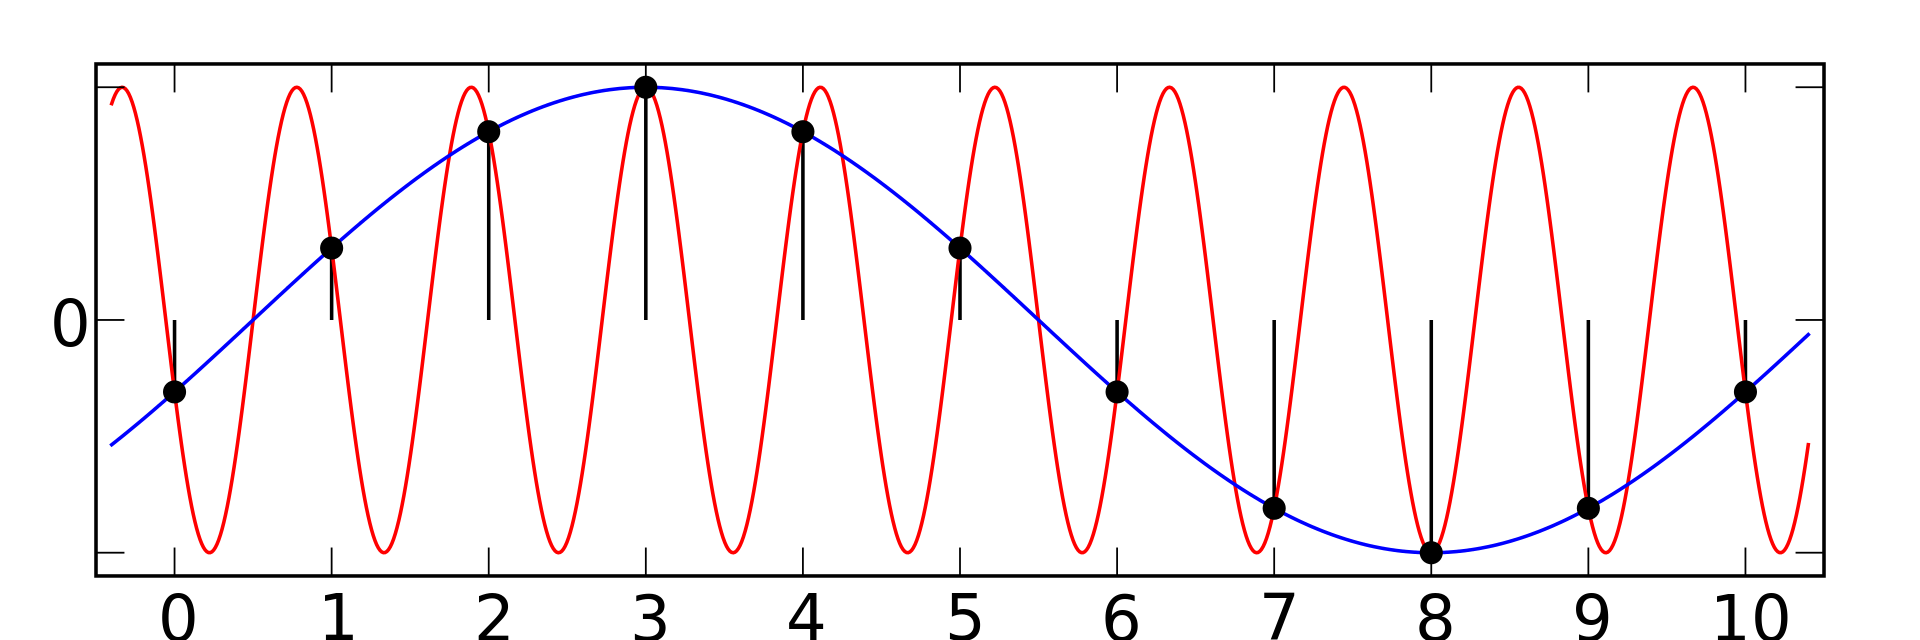
\includegraphics[width=1\textwidth]{Illustrations/AliasingSines.png}
	\caption{Consequences of different sampling rates}
	\label{fig:AliasingSines}
\end{figure}

As we can see in figure \todo{add here nr} if the sampling rate is too small, the signal will be aliased and will get a wrong representation of the signal.

\subsection{Fourier Transform}
As useful as the amplitude might be, for a closer inspection of a signal it is not enough to differentiate human speech from different sound sources. Any sound signal can be recreated from a combination of sinusoidal signals at different frequencies.  For that reason the Fourier Transform can be used to decompose the sound in multiple frequencies. By transforming the signal from the time domain to the frequency domain we can get a lot more information about a specific signal.

\begin{figure}[htp]
	\centering
	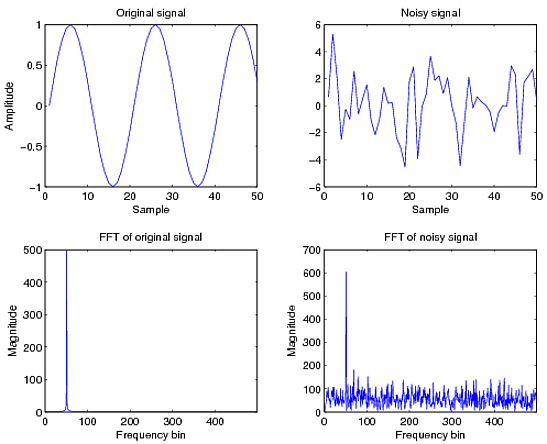
\includegraphics[width=0.7\textwidth]{Illustrations/fftSignals.png}
	\caption{FFT representation of a sine wave and a noisy one}
	\label{fig:fftSignal}
\end{figure}

As we can see in figure \todo{add nr for picture} besides being able to differentiate between different sound sources, especially clean speech, as it was said in a different sections, we know the frequencies in which human voice is so we can see it easier in a frequency domain representation , we can identify noise easier too.

\subsection{Spectrogram of a signal}

